%%%%%%%%%%%%%%%%%%%%%%%%%%%%%%%%%%%%%%%%%%%%%%%%%%%%%%%%%%%%%%%%%%%%%%%%%%%%%%%%
\documentclass[twocolumn]{revtex4}

%%%%%%%%%%%%%%%%%%%%%%%%%%%%%%%%%%%%%%%%%%%%%%%%%%%%%%%%%%%%%%%%%%%%%%%%%%%%%%%%
% Note that comments begin with a "%" and are not turned into text in the .pdf
% document.
%%%%%%%%%%%%%%%%%%%%%%%%%%%%%%%%%%%%%%%%%%%%%%%%%%%%%%%%%%%%%%%%%%%%%%%%%%%%%%%%

%%%%%%%%%%%%%%%%%%%%%%%%%%%%%%%%%%%%%%%%%%%%%%%%%%%%%%%%%%%%%%%%%%%%%%%%%%%%%%%%
% Include some extra packages.
%%%%%%%%%%%%%%%%%%%%%%%%%%%%%%%%%%%%%%%%%%%%%%%%%%%%%%%%%%%%%%%%%%%%%%%%%%%%%%%%
\usepackage[]{graphicx}
%%%%%%%%%%%%%%%%%%%%%%%%%%%%%%%%%%%%%%%%%%%%%%%%%%%%%%%%%%%%%%%%%%%%%%%%%%%%%%%%

%%%%%%%%%%%%%%%%%%%%%%%%%%%%%%%%%%%%%%%%%%%%%%%%%%%%%%%%%%%%%%%%%%%%%%%%%%%%%%%%
\begin{document}

%%%%%%%%%%%%%%%%%%%%%%%%%%%%%%%%%%%%%%%%%%%%%%%%%%%%%%%%%%%%%%%%%%%%%%%%%%%%%%%%
\title{
Human vs. Raptor: Will You Survive?
}

\author{Jada Hawkins-Hill}
\affiliation{Siena College, Loudonville, NY}

\date{\today}

\begin{abstract}
    The purpose of this project is to determine whether a human is able to get away from a raptor using Python coding and the Monte Carlo method. With a head start of 30 meters, a human can only outrun a raptor for two seconds, but once the raptor is one meter from the human, it will begin to attack. There is a 20 percent chance for it to bite the first time, a 15 percent chance the second time, and finally a 7 percent chance the last time before it gives up. Based on the results, there is a 70 percent to 85 percent chance that the human can get away from the raptor.
\end{abstract}

\maketitle
%%%%%%%%%%%%%%%%%%%%%%%%%%%%%%%%%%%%%%%%%%%%%%%%%%%%%%%%%%%%%%%%%%%%%%%%%%%%%%%%

%%%%%%%%%%%%%%%%%%%%%%%%%%%%%%%%%%%%%%%%%%%%%%%%%%%%%%%%%%%%%%%%%%%%%%%%%%%%%%%%
\section{Position vs. Time}
The velociraptor is able to run 18 meters per second, while the human is only able to run three meters per second, so the human is given a 30 meter head start. Therefore the equations used to find their accelerations at any given time is:
$$human = (3t) + 30$$
$$raptor = 18t$$
where t was 100 evenly spaced intervals between 0 and 10 seconds.
A plot of the acceleration of both was then created.
\begin{figure}[h!]
	\centering
	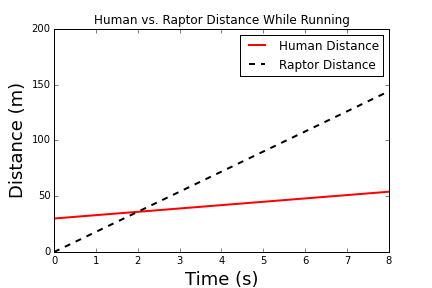
\includegraphics[width=0.5\textwidth]{HVR.png}
	\caption{Human vs. Raptor acceleration. \label{fig:HVR}}
\end{figure}
%%%%%%%%%%%%%%%%%%%%%%%%%%%%%%%%%%%%%%%%%%%%%%%%%%%%%%%%%%%%%%%%%%%%%%%%%%%%%%%%


%%%%%%%%%%%%%%%%%%%%%%%%%%%%%%%%%%%%%%%%%%%%%%%%%%%%%%%%%%%%%%%%%%%%%%%%%%%%%%%%
\section{When Does the Raptor Catch Up to the Human?}
Based on the plot and basic algebra, there is an instant in time when the human and raptor are at the same distance. To algebraically find the time when they cross paths, the two equations for the human and raptor must equal each other:
$$(3t) + 30 = 18t$$

Subtracting 3t from both sides will result in:
$$30 = 15t$$
And dividing by 15 on both sides will result in the time being two seconds. While this is a good way to approach the problem, it is not how it should be used to solve with Python.

To find the time using Python, I created a loop that took both equations and turned them into integers that way it could drop the decimals and give an approximate answer for distance in meters. When the decimals are dropped, I made a conditional "if" statement that created a boolean of both variables; if the human distance, h, is the same as the raptor distance, r, then it should print "The raptor catches up to the human at t seconds when they are both at h meters, but the human has only ran h - 30 meters.

When executed, the time the two are at the same distance is at 2.02 seconds when they are both at 36 meters, but the human has only ran six meters from the start.

\section{When is it Close Enough to Strike?}
Now it is said that the raptor will not start attacking the human until it is one meter behind him. To figure this out, I took the same equations from the beginning and made them integers once again. Once they were integers, I created a new variable named "one" to be equal to the human's distance minus the raptor's distance. Upon finding that there was a distance of one meter between the two, I made an "if" conditional of a boolean to state that when "one" is equal to one, it will assign the raptor's distance to a new variable called "one meter", and will then change this number back into an array.

When the code is executed, it shows that it takes 1.9 seconds for the raptor to be at 34 meters, which is one meter behind the human, while the human has only ran five meters at that time. A plot, indicating when the raptor is one meter away with an arrow, was then created.

\begin{figure}[h!!!]
	\centering
	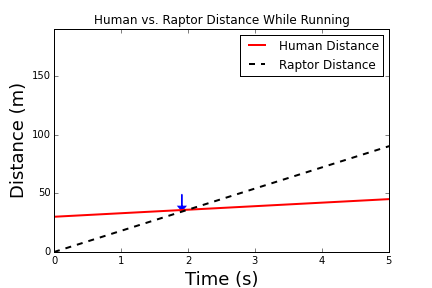
\includegraphics[width=0.5\textwidth]{HVR_new.png}
	\caption{The arrow indicates when the raptor is one meter away, indicating where it will begin to attack the human. \label{fig:HVR_new}}
\end{figure}

\section{Will it Bite the Human?}
The raptor will attack when it is one meter behind, but it will try to bite the human only three times. For the first try, there is only a 20 percent chance that it will bite him. The second time, there is only a 15 percent chance. Finally, the third try, there is only a 7 percent chance. That means that the human has an 80 percent chance to live the first time, 85 percent the second time, and 93 percent the last time!

I made a separate variable outside of the nested conditional that would keep track of the times the human was able to escape from the raptor, then used a variable called "times" to use as part of a loop. A "for" loop was created that ranged from zero to the amount assigned with "times," which was 1000 to get a better probability.

In order to figure out what the probability is that the person will get away, I had to create a variable called "chance" that was able to generate random numbers between zero and one. Inside of a nested "if" conditional, I then made it so that if the number generated by "chance" was less than or equal to .8 (the 80 percent chance that the human has to live), then it would print out "You were able to not to get bit by the raptor!" or else it would print out "You were eaten by the raptor." If the number generated was less than .8 and the human did not get bit, it went on to the next "if" statement that said if the number was less than .85, it would print "You did it again!" otherwise it would print "You were only able to get away once." Finally, if the human was able to get away both times and the number is below .93, then it would print "You were able to get away from the raptor!" otherwise it would print "You did not make it."

The code was executed 1000 times, and the results show that the human was able to get away from the raptor anywhere between 705 to 820 times, which would give a 70.5 percent to 82 percent chance that the human is able to escape.
%%%%%%%%%%%%%%%%%%%%%%%%%%%%%%%%%%%%%%%%%%%%%%%%%%%%%%%%%%%%%%%%%%%%%%%%%%%%%%%%

%%%%%%%%%%%%%%%%%%%%%%%%%%%%%%%%%%%%%%%%%%%%%%%%%%%%%%%%%%%%%%%%%%%%%%%%%%%%%%%%
\end{document}
%%%%%%%%%%%%%%%%%%%%%%%%%%%%%%%%%%%%%%%%%%%%%%%%%%%%%%%%%%%%%%%%%%%%%%%%%%%%%%%%
